\documentclass[UTF8,ctexart,a4paper,11pt,openany]{article}
\usepackage[slantfont,boldfont]{xeCJK}
\usepackage{fontspec}
\usepackage{ctex}

\setCJKmainfont{SimSun}%[BoldFont=SimHei] %去掉注释：bf字体为黑体

\setsansfont{SimHei}
\setCJKsansfont{SimHei}

\xeCJKsetcharclass{"2160}{"2470}{1}% 1: CJK
\xeCJKsetup{AutoFallBack=true}
\setCJKfallbackfamilyfont{\CJKrmdefault}{SimSun.ttf}

%\setmainfont{Times New Roman}     %去掉注释：Times new roman字体
%\usepackage{mathptmx}             %去掉注释：Times new roman字体

\usepackage{mathtools}
\usepackage{amsmath}
\usepackage{amsfonts}
\usepackage{amssymb}
\usepackage{amsthm}
\usepackage[T1]{fontenc}
\usepackage{indentfirst} %段首空两格

\usepackage{graphicx}
\usepackage{geometry}
\usepackage{latexsym}
\usepackage{fancyhdr}
\usepackage{epstopdf}
%\usepackage{pifont}
%\usepackage[perpage,symbol*]{footmisc}
\usepackage{titlesec}
\usepackage{setspace}
\usepackage{enumerate}
\usepackage{enumitem}
\usepackage{multicol}
\usepackage{url}
\usepackage{exscale}
\usepackage{ulem}
\usepackage{relsize}
\usepackage{mathrsfs}
\usepackage{tikz}
\usepackage{wrapfig}
\usepackage{framed}
\usepackage{bm}
%\usepackage{pstricks,pst-node,multido,ifthen,calc}
\usepackage[all]{xy}
\usepackage{extarrows}
%\usepackage[backref]{hyperref}
\usepackage{hyperref}
\usepackage{stfloats} %插图的时候不分页

\setlength{\parindent}{2em} %段首空两格
\linespread{1.2}
\usepackage{listings}
\usepackage{xcolor}
\usepackage{algorithm}
\usepackage{algorithmicx}
\usepackage{algpseudocode}
\usepackage{mdframed}
\usepackage{extarrows}
\usepackage{diagbox}
\usepackage{makecell}

\theoremstyle{definition}
\mdfdefinestyle{theoremstyle}{%
linecolor=green!40,linewidth=.5pt,%
backgroundcolor=green!10,
skipabove=8pt,
skipbelow=5pt,
innerleftmargin=7pt,
innerrightmargin=7pt,
frametitlerule=true,%
frametitlerulewidth=.5pt,
frametitlebackgroundcolor=green!35,
frametitleaboveskip=0pt,
frametitlebelowskip=0pt,
innertopmargin=.4\baselineskip,
innerbottommargin=.4\baselineskip,
shadow=true,shadowsize=3pt,shadowcolor=black!20,
%theoremseparator={\hspace{1pt}},
theoremseparator={.},
nobreak=true,
}


\everymath{\displaystyle}

\newtheorem{definition}{\hspace{2em}定义}[section]
\newtheorem{axiom}{\hspace{2em}公理}

\mdtheorem[style=theoremstyle]{theorem}{定理}
\mdtheorem[style=theoremstyle]{example}{例}
\mdtheorem[style=theoremstyle]{exercise}{问题}
\newtheorem{lemma}[theorem]{\hspace{2em}引理}
\newtheorem{corollary}[theorem]{\hspace{2em}推论}

\newcommand*{\QED}{\hfill\ensuremath{\square}}
\newcommand*{\rmk}{\textbf{注：}}
\renewcommand*{\proof}{\textbf{证明：}}
\newcommand*{\tips}{\textbf{提示：}}
\newcommand*{\hard}{\textbf{\color{red}(难)}}
\newcommand*{\eqsmall}{\setlength\abovedisplayskip{1pt}\setlength\belowdisplayskip{1pt}}
\geometry{left=2cm,right=2cm,top=2cm,bottom=2cm}
\title{数值分析上机报告（示例）}
\author{Fiddie}
\pagestyle{fancy}
\fancyfoot[C]{}
\fancyhead[RO]{ \thepage}
\fancyhead[LE]{\thepage  }
\fancyhead[RE]{\rightmark (学号：201145149 ，姓名：Fiddie)}
\fancyhead[LO]{\leftmark (学号：201145149 ，姓名：Fiddie)}
\titleformat{\chapter}{\centering\huge\bfseries}{第\,\thechapter\,章}{1em}{} %更改标题样式
\titleformat{\section}{\bfseries\Large}{$\S$\,\thesection\,}{1em}{} %更改标题样式
\titlespacing*{\chapter}{0pt}{9pt}{0pt} %调整标题间距
\setenumerate[1]{itemsep=0pt,partopsep=0pt,parsep=\parskip,topsep=0pt} %设置enumerate行间距
\setenumerate[2]{itemsep=0pt,partopsep=0pt,parsep=\parskip,topsep=0pt} %设置enumerate行间距
\setitemize[1]{itemsep=0pt,partopsep=0pt,parsep=\parskip,topsep=0pt} % 设置itemize行间距
\setlist[enumerate,2]{label=(\arabic*),topsep=0mm,itemsep=0mm,partopsep=0mm,parsep=\parskip}
    % 设置二层枚举为(1)样式
    
\newfontfamily\hei{SimHei}
\newcommand\textcf[1]{\textbf{\textsf{\hei{#1}}}}

\newcommand\e{\leftarrow}
%\renewcommand{\bibname}{参考文献}

\begin{document}

\begin{center}
{\huge \textbf{数值计算第一周上机(示例)特别说明}}

修订日期：2025年2月17日
\end{center}

可以观看FiddieMath视频\url{https://www.bilibili.com/video/BV1JF411W797}

\noindent \textbf{上机报告要素：}

1．问题：展现上机作业要解决的问题，或者实际问题的背景．

2．算法原理与描述：结合你的理解，展现上机作业要求实现的算法的思想或推导、算法步骤．

（\rmk 很欢迎同学们引入本课程教材之外的算法与作业要求的算法作比较，出自别的教材、论文，或者同学们自己提出新算法均可．）

3．输出结果分析：把算法应用于具体问题时，会有输出结果，把这些输出结果用合适的方式展示出来，可以用表格呈现，也可以画图呈现．如果画图呈现，一般画图在一页纸范围内呈现，如果图片太多就放到附录．可以展示的内容包括：误差曲线图、输出结果图、算法的收敛率、内存占用、计算速度（例如重复运行10000次分别用时多少）、算法的稳定性．

4．结论：把输出结果分析得出的结论、几种算法的各方面优劣对比等展现出来．

5．(可选)参考文献：如果你引入了课程教材之外的内容，请在文末附上参考文献．

\vspace{0.5cm}

\noindent \textbf{补充说明：}

1．评分标准：完成度低的得$0\sim 5$分，然后根据完成质量情况赋$6\sim 10$分．其中，上机问题基本回答正确，且可读性强、展现简洁清晰的可得10分．如果上机报告有非常大的亮点，瑕不掩瑜，也可以获得加分．

2．代码、输出一大堆的数据都放在附录，而少量数据、图片可以放在正文．\textbf{同一坐标系中的多条曲线请在同一张图中用不同的图例画出来．}

3．实验报告不是越长越好，而是信息量越大越好.

4．算法和代码尽量减少重复冗余，比如用两个不同的终止准则的时候不需要写两次算法或者代码(因为它们只是在终止准则的部分作了小改动)．

5．请保证你的实验报告的排版整洁，比如字体尽量用同一种，字号保持一致，行距采用不超过1.25倍的行距 (如果用1.5倍行距就会显得过于空白了，并且算法和代码的呈现占了好几页篇幅).

6．如果有多张图片是相似的（例如只是改动一个参数就又画了一个图），请改为紧凑排列（一行放多张图），或者把几条曲线放在一起，旁边附上图例．示例：\cite{MScaleDNN2020}

\begin{center}
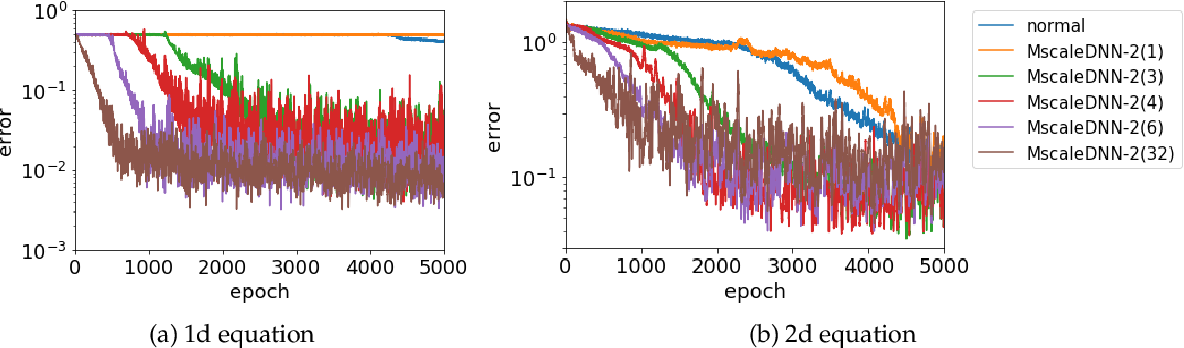
\includegraphics[width=0.9\textwidth]{pics/14-Figure10-1.png}
\end{center}


\clearpage

\begin{center}
{\huge \textbf{数值分析第一周上机作业(示例)}}

{\large 学号：201145149，姓名：Fiddie}
\end{center}

\section{问题}

	利用区间分半法求解方程$x^3-3.2x^2-0.1x+4=0$，使误差不大于$ 10^{-7}$：\par
(1)考虑不同的终止原则；\par
(2)分析误差与收敛速度．



\section{算法思路}

初步分析：可见$ f(0)f(2) < 0$，且$f'(x)$在$[0,2]$上不变号．于是$f(x)$在目标区间中
单调且有且仅有一个零点，方便使用区间半分法求解．

\begin{figure}[htbp]
\centering
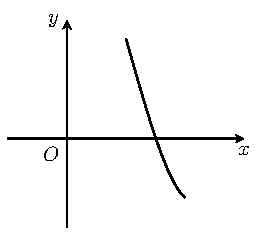
\includegraphics{pics/pic4.pdf}
\caption{函数$f(x)=x^3-3.2x^2-0.1x+4$在$[1,2]$上的图像}
\label{graph:1}
\end{figure}


对于闭区间$[a,b]$内的连续函数$f(x)$，如果有$f(a)f(b)<0$，由介值定理，$f(x)$在$[a,b]$内必有一根$x^*$．我们可以考虑对该区间折半，不断缩小范围，最后得到方程$f(x)=0$的数值解$\tilde{x}$，并且满足一定的精度，即$|x^*-\tilde{x}|<\varepsilon$．理论上这由闭区间套定理保证．


\begin{algorithm}
    \caption{区间分半法}
    \begin{algorithmic}[1] %每行显示行号
        \Require 区间$[a,b]$，终止误差$\varepsilon$，最大迭代次数$m$.
        \Ensure 近似解$ p$或失败信息.
        \Function {Bisection}{$a,b,\varepsilon$}
            \State $e\e b-a,\ u\e f(a),\ v\e f(b)$
            \For {$k=1,\cdots,m$}
                \State $ e\e e/2,\ p\e a+e,\ w\e f(p)$；
                \If {终止准则满足}
                    \State 输出$p$，结束程序.
                \EndIf
                \State 若$wv<0$，则$ a\e p,\ u\e w$; 否则$ b\e p,\ v\e w$.
            \EndFor
            \State 输出失败信息.
        \EndFunction
    \end{algorithmic}
\end{algorithm}

其中，在算法1中，终止准则可以取为$|w|<\varepsilon$或者$|e|<\varepsilon$.
相关的代码见附录部分.


\section{结果分析}%重点（误差图、结果图、分析算法的收敛性（速度）、内存使用（时间、空间）、计算量、稳定性

第一种终止原则和第三种终止原则在终止时都迭代了25步，得到了相同的结果：1.5085067；而第二种终止原则迭代了24步，得到了一个精度稍差的结果：1.508507．

由于迭代过程相同，每种终止原则所得迭代序列都是一样的，所以以下仅分析迭代25步所得结果．略微修改C++程序，输出每一步迭代得到的$ x_n$的值，同时进一步迭代15 次以得到近似精确值$p$．用excel进行数据处理，计算出绝对误差并取对数，得到数据表如表 \ref{tab:data} 所示(见附录部分)．在此基础上，根据迭代序列作出散点图如图 \ref{graph:1} 所示．

\begin{figure}[htbp]
\centering
\begin{minipage}{0.48\textwidth}
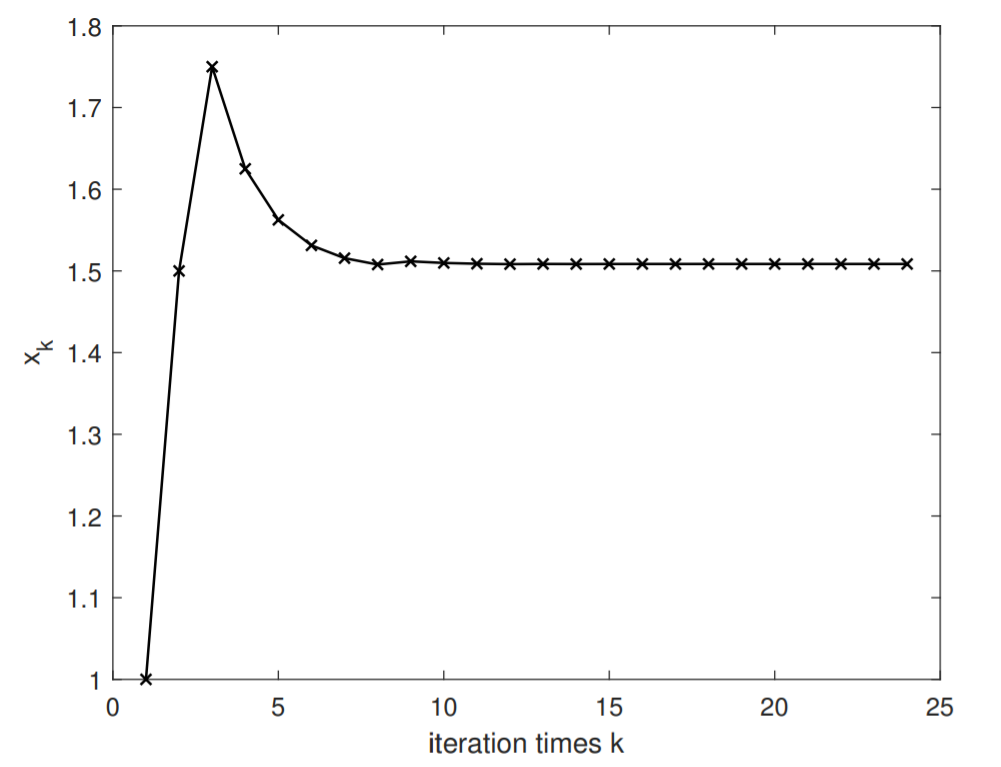
\includegraphics[width=1\textwidth]{pics/pic3.png}
\caption{迭代序列散点图}
\label{graph:1}
\end{minipage}
\end{figure}

\begin{figure}[htbp]
\centering
\begin{minipage}{0.48\textwidth}
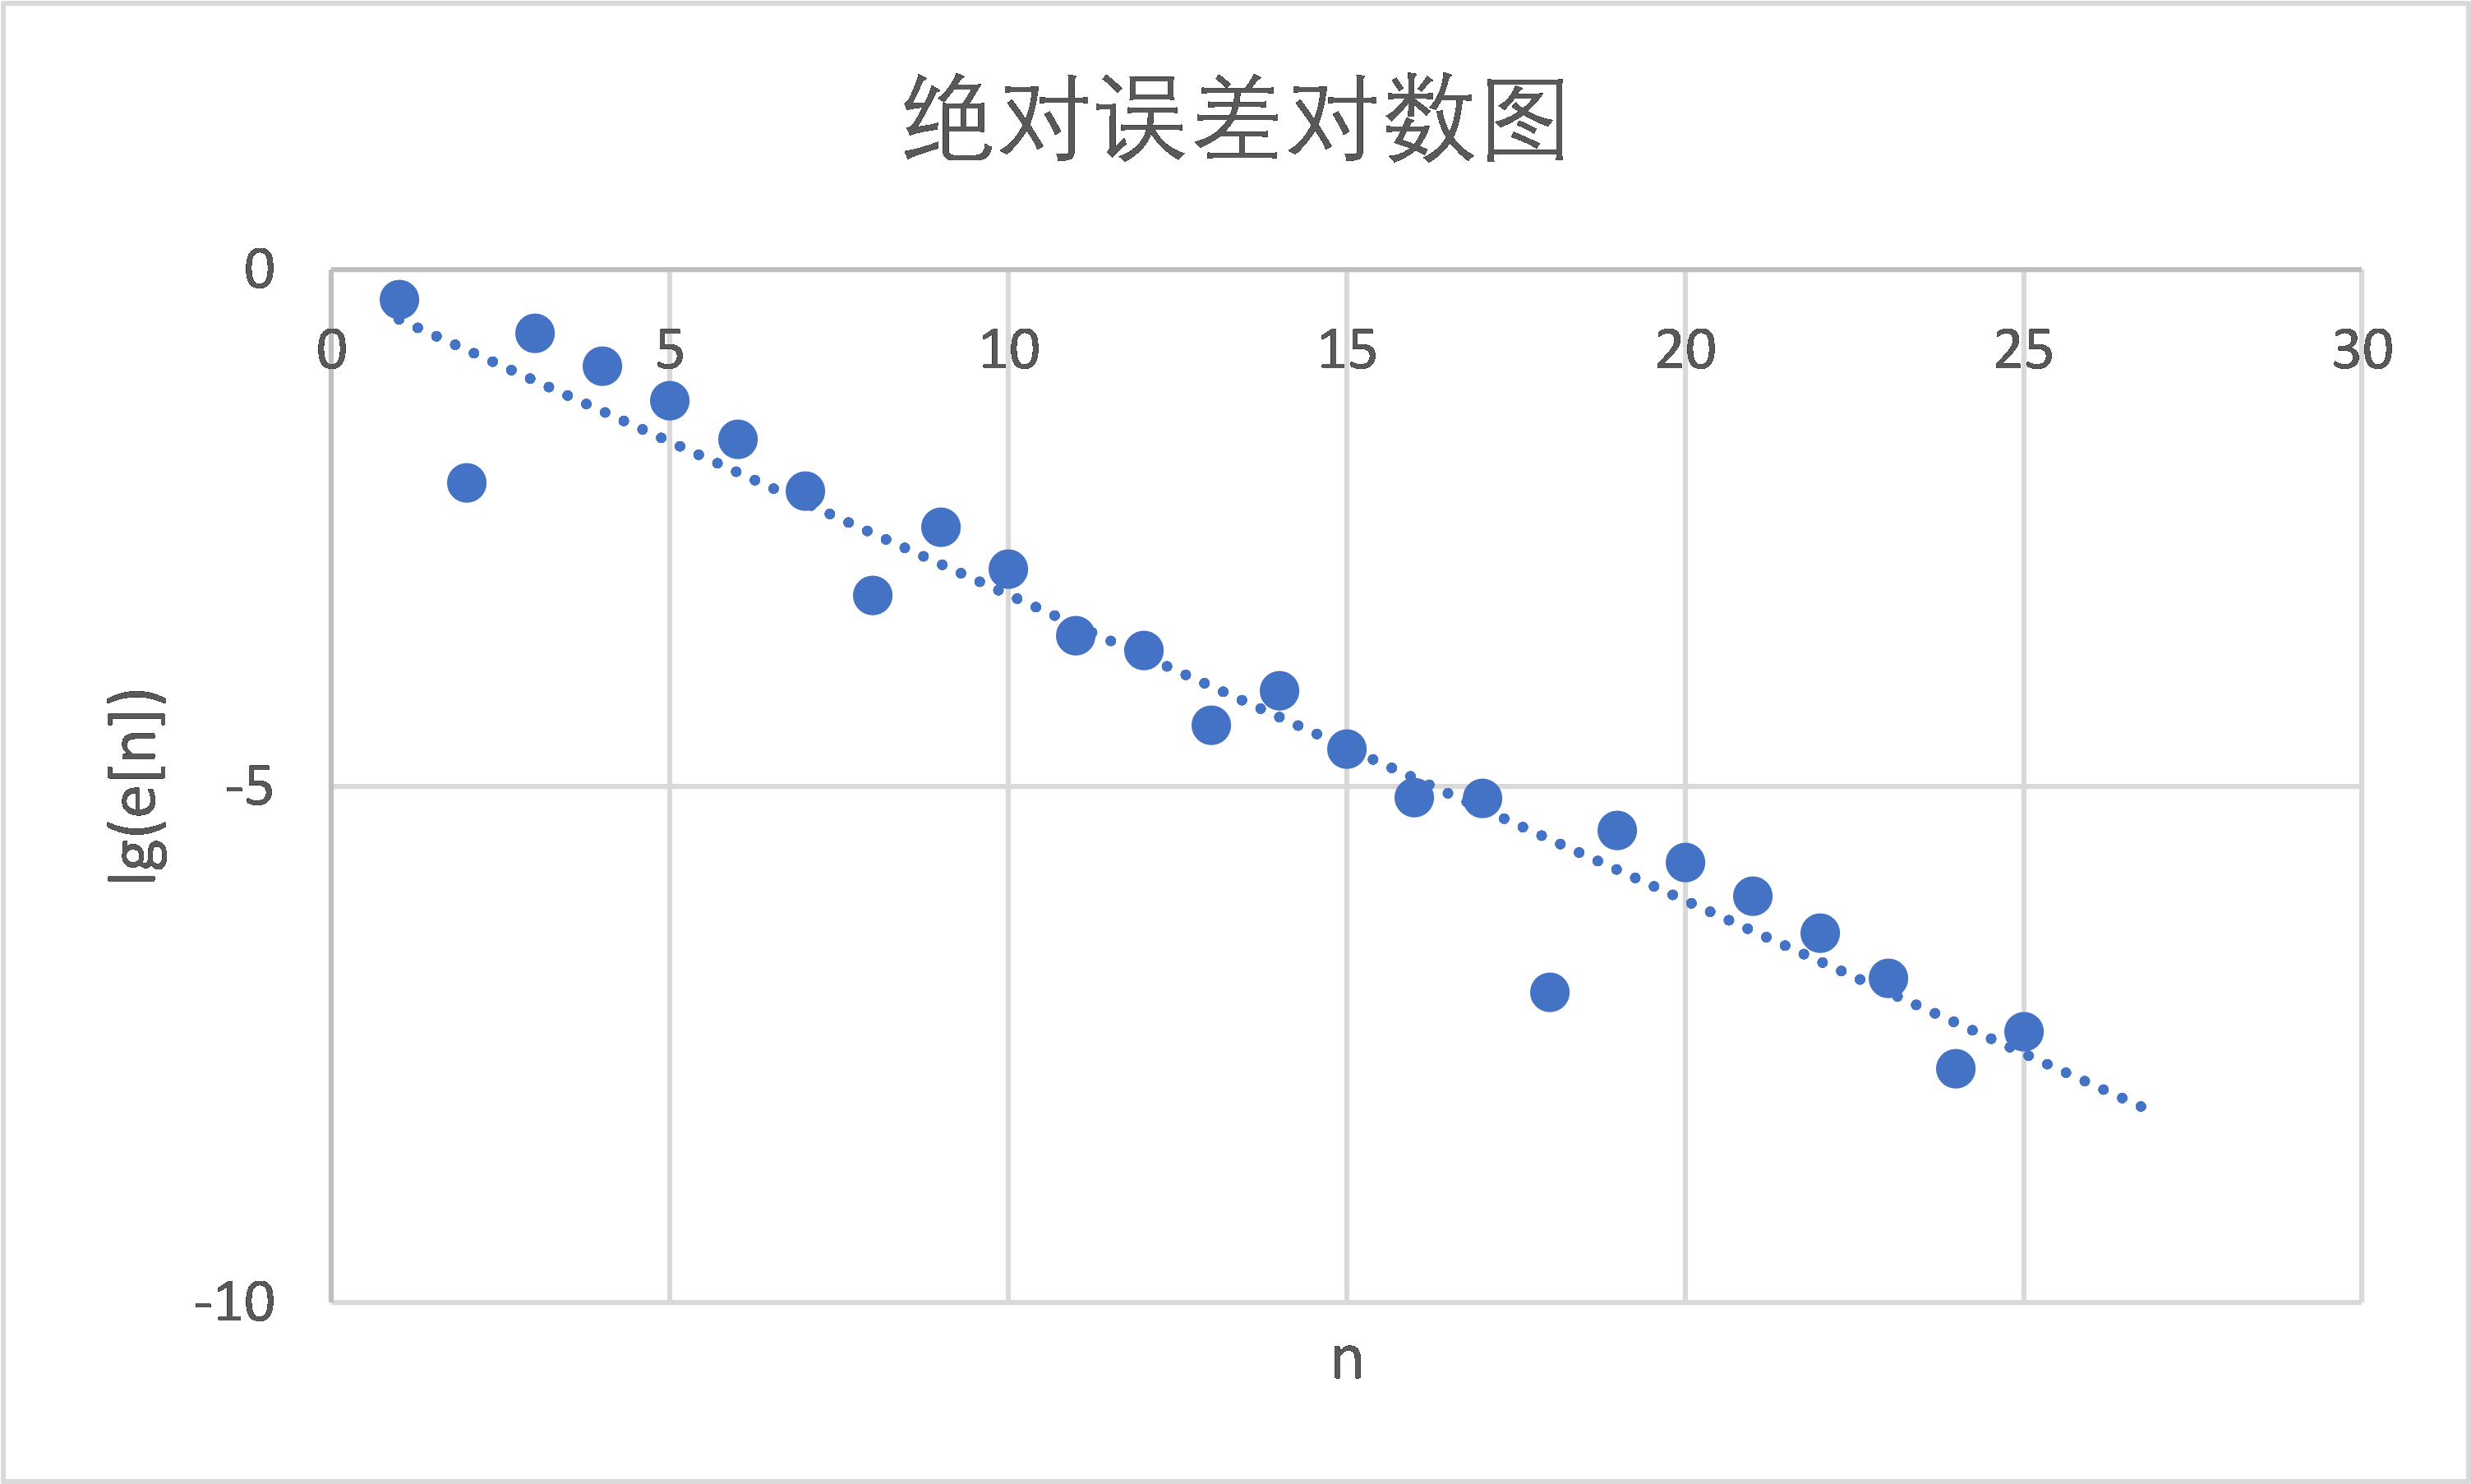
\includegraphics[width=1\textwidth]{pics/pic1.png}
\caption{绝对误差对数图}
\label{graph:2}
\end{minipage}
\end{figure}

由图 \ref{graph:1} 可知，在坐标轴固定的情况下，初始值经过8次迭代就趋于一个稳定的值了，由此可粗略看出二分法的迭代速度是比较快的．为了进一步分析算法的收敛性，我们作出绝对误差以10为底的对数随$ n$变化的散点图如图 \ref{graph:2} 所示，图中穿过散点的虚线是经过线性回归分析得到的回归直线$ \lg e_n=-0.296n-0.181$．结果显示$ R^2=0.949$，与1仅差$ 5\%$．再结合图象特征，我们有很大的把握得出$ \lg e_n$与$ n$之间的线性关系．因此二分法是线性收敛的，并且根据回归直线，我们有
$$ \lg \frac{e_{n+1}}{e_n}=\lg e_{n+1}-\lg e_n\simeq-0.296\Rightarrow \frac{e_{n+1}}{e_n}\simeq 10^{-0.296}\simeq0.506.$$

\section{结论}

总得来看，该算法\textbf{结构较为简单}，且只用到了函数的连续性，\textbf{适用范围大}. 另外算法\textbf{稳定性高}，只要符合$f(a)f(b) < 0$就可以使用，且一定会收敛. 在不知道确切信息的情况下，很适合用来求得根的近似值，在此基础上用更高阶的方法来进一步加强根的精度．

但是该算法没有利用函数更多的性质（如导数、二阶导数等），收敛速度呈线性，\textbf{收敛速度较慢}．另外，由于只能通过半分区间来进行迭代，\textbf{该算法不是每一步都会带来一个函数值稳定的下降}（迭代点和最终解之间的距离也不会稳定的下降）．此外，该方法只适用于单值函数，\textbf{对于向量值函数和多元函数无法推广}．

\clearpage

\section{附录: 程序代码}

\textbf{说明：}展示关键算法部分的代码及算例即可．

\lstset{
    numbers=left,
    language=C++,
    keywordstyle=\color{blue!100},
    commentstyle=\color{green!50!blue!50!},
    frame=shadowbox，%阴影
    escapeinside=''，%英文分号输入中文
    xleftmargin=2em，xrightmargin=2em,aboveskip=1em,
    framexleftmargin=2em,
    extendedchars=false}

\begin{lstlisting}[aboveskip=0pt]
inline double f(double x)
{
    return 4+x*(-0.1+x*(-3.2+x));
}
int main()
{
    int m=30;
    double a=0,b=2,Tol=1e-7;
    double e=b-a,u=f(a),v=f(b),w,p;
    int k;
    for(k=1;k<=m;k++){
        e=e/2;
        p=a+e;
        w=f(p);
        if(fabs(w)<Tol){ // OR: e<Tol
            cout<<setprecision(10)<<p<<endl;
            return 0;
        }
        if(w*v<0){ a=p; u=w; } else{ b=p; v=w; }
    }
    cout<<"Method failed."<<endl;
    return 0;
}
\end{lstlisting}

\clearpage

\section{附录：迭代输出结果}

\textbf{说明：}为保证正文的简洁可读，对于大量的数据请在附录给出．


% Table generated by Excel2LaTeX from sheet '确定步数'
\begin{table}[htbp]
\centering
\caption{迭代数据表}
\begin{tabular}{|lllll|}\hline
$ n$     & $ x_n$  & $ p(n=40)$     & $ |p-x_n|=e_n$ &  $ \lg e_n$ \\\hline
1     & 1     & 1.508506674 & 0.508506674 & -0.293703343 \\
    2     & 1.5   &       & 0.008506674 & -2.070240213 \\
    3     & 1.75  &       & 0.241493326 & -0.617094867 \\
    4     & 1.625 &       & 0.116493326 & -0.933698955 \\
    5     & 1.5625 &       & 0.053993326 & -1.267659919 \\
    6     & 1.53125 &       & 0.022743326 & -1.643146022 \\
    7     & 1.515625 &       & 0.007118326 & -2.147622123 \\
    8     & 1.5078125 &       & 0.000694174 & -3.158531695 \\
    9     & 1.51171875 &       & 0.003212076 & -2.493214179 \\
    10    & 1.509765625 &       & 0.001258951 & -2.899991152 \\
    11    & 1.508789063 &       & 0.000282389 & -3.5491529 \\
    12    & 1.508300781 &       & 0.000205893 & -3.686359074 \\
    13    & 1.508544922 &       & 3.82479E-05 & -4.417392 \\
    14    & 1.508422852 &       & 8.38224E-05 & -4.076640029 \\
    15    & 1.508483887 &       & 2.27872E-05 & -4.642308644 \\
    16    & 1.508514404 &       & 7.73036E-06 & -5.111800419 \\
    17    & 1.508499146 &       & 7.52843E-06 & -5.123295496 \\
    18    & 1.508506775 &       & 1.00963E-07 & -6.995837711 \\
    19    & 1.50850296 &       & 3.71373E-06 & -5.430189176 \\
    20    & 1.508504868 &       & 1.80639E-06 & -5.743189533 \\
    21    & 1.508505821 &       & 8.52711E-07 & -6.069197977 \\
    22    & 1.508506298 &       & 3.75874E-07 & -6.424957541 \\
    23    & 1.508506536 &       & 1.37456E-07 & -6.861837657 \\
    24    & 1.508506656 &       & 1.82463E-08 & -7.738825664 \\
    25    & 1.508506715 &       & 4.13584E-08 & -7.38343669 \\\hline
\end{tabular}%
\label{tab:data}%
\end{table}%

\clearpage

\bibliographystyle{unsrt}
\bibliography{Reference}
\end{document}




















